\documentclass[a4paper,20pt]{article}
\usepackage{amsmath,amssymb,epsf,epsfig,times}
\usepackage{multicol}
\usepackage[all]{xy}
\usepackage{color}
\usepackage{ctex}
\usepackage{subfigure}
\usepackage{url,cite}
\usepackage{tikz}
\usepackage[english]{babel}
\usepackage[utf8]{inputenc}

\usepackage{pdfpages}

%\usepackage{caption}
%
%\usepackage[font=small,labelfont=bf,labelsep=none]{caption}
\usepackage[font=default,labelfont=bf,labelsep=period]{caption}

\usepackage{makecell}
\usepackage{booktabs} %引入三线表
\usepackage{diagbox}
\usepackage{multirow}

\usepackage{fancyhdr}
\usepackage{float}
\usepackage{ulem}

\usepackage{listings}
\usepackage{xcolor}

\usepackage{enumerate}
\lstset{
    basicstyle          =   \sffamily,          % 基本代码风格
    keywordstyle        =   \bfseries,          % 关键字风格
    commentstyle        =   \rmfamily\itshape,  % 注释的风格,斜体
    stringstyle         =   \ttfamily,  % 字符串风格
    flexiblecolumns,                % 别问为什么,加上这个
    numbers             =   left,   % 行号的位置在左边
    showspaces          =   false,  % 是否显示空格,显示了有点乱,所以不现实了
    numberstyle         =   \zihao{-5}\ttfamily,    % 行号的样式,小五号,tt等宽字体
    showstringspaces    =   false,
    captionpos          =   t,      % 这段代码的名字所呈现的位置,t指的是top上面
    frame               =   lrtb,   % 显示边框
}
\lstdefinestyle{Python}{
    language        =   Python, % 语言选Python
    basicstyle      =   \zihao{-5}\ttfamily,
    numberstyle     =   \zihao{-5}\ttfamily,
    keywordstyle    =   \color{blue},
    keywordstyle    =   [2] \color{teal},
    stringstyle     =   \color{magenta},
    commentstyle    =   \color{red}\ttfamily,
    breaklines      =   true,   % 自动换行,建议不要写太长的行
    columns         =   fixed,  % 如果不加这一句,字间距就不固定,很丑,必须加
    basewidth       =   0.5em,
}

\newtheorem{theorem}{Theorem}[section]
\newtheorem{lemma}{Lemma}[section]
\def\proof{\noindent{\it Proof: }}
\def\QED{\mbox{\rule[0pt]{1.5ex}{1.5ex}}}
\def\endproof{\hspace*{\fill}~\QED\par\endtrivlist\unskip}
\newcommand{\re}{\mathbb{R}}
\def\sV{\mathcal{V}}
\def\sS{\mathcal{S}}
\def\sQ{\mathcal{Q}}

\newcommand{\mc}{\mbox{: }}

\newcommand{\normsq}[1]{\left\|#1\right\|^2}
\newcommand{\norm}[1]{\left\|#1\right\|}
%\newcommand{\sgn}[1]{\mbox{sgn}(#1)}
\newcommand{\pde}[2]{\frac{\partial #1}{\partial #2}}
\newcommand{\fundef}[3]{#1:#2\to #3}
\newcommand{\abs}[1]{\left|#1\right|}
\newcommand{\mymatrix}[2]{\left(\begin{array}{#1}#2\end{array}\right)}
\newcommand{\defeq}{\stackrel{\triangle}{=}}
\newcommand{\paren}[1]{\left(#1\right)}
%\theoremstyle{plain} \newtheorem{theorem}{Theorem}
%\theoremstyle{plain} \newtheorem{algorithm}{Algorithm}
\newtheorem{axiom}[theorem]{Axiom}
\newtheorem{definition}[theorem]{Definition}
\newtheorem{assumption}[theorem]{Assumption}
\newtheorem{example}[theorem]{Example}
%\theoremstyle{plain}\newtheorem{lemma}{Lemma}
%\newtheorem{proposition}[theorem]{Proposition}
\newtheorem{remark}[theorem]{Remark}
\newtheorem{corollary}[theorem]{Corollary}

\newcommand{\Acal}{\mathcal{A}}
\newcommand{\Bcal}{\mathcal{B}}
\newcommand{\Ccal}{\mathcal{C}}
\newcommand{\Dcal}{\mathcal{D}}
\newcommand{\Ecal}{\mathcal{E}}
\newcommand{\Fcal}{\mathcal{F}}
\newcommand{\Gcal}{\mathcal{G}}
\newcommand{\Hcal}{\mathcal{H}}
\newcommand{\Ical}{\mathcal{I}}
\newcommand{\Jcal}{\mathcal{J}}
\newcommand{\Kcal}{\mathcal{K}}
\newcommand{\Lcal}{\mathcal{L}}
\newcommand{\Mcal}{\mathcal{M}}
\newcommand{\Ncal}{\mathcal{N}}
\newcommand{\Ocal}{\mathcal{O}}
\newcommand{\Pcal}{\mathcal{P}}
\newcommand{\Qcal}{\mathcal{Q}}
\newcommand{\Rcal}{\mathcal{R}}
\newcommand{\Scal}{\mathcal{S}}
\newcommand{\Tcal}{\mathcal{T}}
\newcommand{\Ucal}{\mathcal{U}}
\newcommand{\Vcal}{\mathcal{V}}
\newcommand{\Wcal}{\mathcal{W}}
\newcommand{\Xcal}{\mathcal{X}}
\newcommand{\Ycal}{\mathcal{Y}}
\newcommand{\Zcal}{\mathcal{Z}}


\def\omegavec{\boldsymbol{\omega}}
\newcommand{\alphabf}{\boldsymbol{\alpha}}
\newcommand{\omegabf}{\boldsymbol{\omega}}
\def\omegavec{\boldsymbol{\omega}}
\newcommand{\taubf}{\boldsymbol{\tau}}
\newcommand{\qbf}{\mathbf{q}}
\newcommand{\ybf}{\mathbf{y}}
\newcommand{\pbf}{\mathbf{p}}
\newcommand{\rbf}{\mathbf{r}}
\newcommand{\ebf}{\mathbf{e}}
\newcommand{\onebf}{\mathbf{1}}
\newcommand{\zerobf}{\mathbf{0}}
\newcommand{\abf}{\mathbf{a}}
\newcommand{\ibf}{\mathbf{i}}
\newcommand{\jbf}{\mathbf{j}}
\newcommand{\kbf}{\mathbf{k}}
\newcommand{\vbf}{\mathbf{v}}
\newcommand{\wbf}{\mathbf{\omega}}
\newcommand{\fbf}{\mathbf{f}}
\newcommand{\zbf}{\mathbf{z}}
\newcommand{\xbf}{\mathbf{x}}
\newcommand{\dbf}{\mathbf{d}}
\newcommand{\Rbf}{\mathbf{R}}
\newcommand{\Tbf}{\mathbf{T}}

\newcommand{\Cbf}{\mathbf{C}}
\newcommand{\Ibf}{\mathbf{I}}
\newcommand{\Pbf}{\mathbf{P}}
\newcommand{\Qbf}{\mathbf{Q}}
\newcommand{\Vbf}{\mathbf{V}}
\newcommand{\Jbf}{\mathbf{J}}
\newcommand{\Xbf}{\mathbf{X}}
\newcommand{\Abf}{\mathbf{A}}
\newcommand{\Kbf}{\mathbf{K}}
\newcommand{\Gammabf}{\boldsymbol{\Gamma}}
\newcommand{\nubf}{\boldsymbol{\nu}}
\newcommand{\xibf}{\boldsymbol{\xi}}
\newcommand{\Xibf}{\boldsymbol{\Xi}}
\newcommand{\Omegabf}{\boldsymbol{\Omega}}


\newcommand{\ubf}{\mathbf{u}}

\newcommand{\lth}{\ell{\text{th}}}
\newcommand{\ith}{i{\text{th}}}
\newcommand{\jth}{j{\text{th}}}
\newcommand{\kth}{k{\text{th}}}
\newcommand{\ip}[2]{\left<#1,~#2\right>}

\newcommand{\OMIT}[1]{}
\title{}
\author{}
\date{}


\pagestyle{fancy}
\fancyhf{}
\chead{\textbf{关于$\lceil$\textcolor{red}{“线性规划”}$\rfloor$的matlab讲解}}
\lhead{魔力铠甲}
\rfoot{Page \thepage}
\begin{document}
\renewcommand{\lstlistlistingname}{代码汇总}
\renewcommand{\lstlistingname}{代码}
\captionsetup[figure]{labelfont={bf},labelformat={default},labelsep=period,name={图}}
\renewcommand\tablename{表}
    总所周知,线性规划是最易理解的应用算法。那么今天来做第一篇算法讲解,首先,这玩意我打算做成期刊,这样多少都能督促自己做完matlab算法。
    \section{线性规划-简介}
    线性规划就是在一组线性约束条件[记为 s.t.(即 subject to)]下,求线性目标函数(通常时决策变量的线性函数)的最大或者最小值。(要求所有的变量都是一次方)
    \par \textbf{八股文:}在人们的生产实践中,经常会遇到如何利用现有资源来安排生产,以取得最大经济
    效益的问题。此类问题构成了运筹学的一个重要分支—数学规划,而线性规划(Linear 
    Programming 简记 LP)则是数学规划的一个重要分支。自从 1947 年 G. B. Dantzig 提出
    求解线性规划的单纯形方法以来,线性规划在理论上趋向成熟,在实用中日益广泛与深
    入。特别是在计算机能处理成千上万个约束条件和决策变量的线性规划问题之后,线性
    规划的适用领域更为广泛了,已成为现代管理中经常采用的基本方法之一。
    \subsection{有限的条件,最大的收益}
    \par \textbf{例题:}张麻子既要攻碉楼又要追替身,他们一伙6人,总共1200法子弹补给;每有一人攻击碉楼就会带来40点士气,每有一人追替身就会带来30点士气;攻碉楼每人需要240发子弹,追替身没人需要120发子弹.问,追碉楼和追替身各派几人,能使士气最大。
   
    \par \small{解:}
    \begin{table}[h]
        
        \caption{模型假设}
        \centering
        \begin{tabular}{ c l }
        \hline
        决策变量 & 实际意义 \\
        \hline
        $x_1$ & 攻碉楼人数\\
        \hline
        $x_2$ & 追替身人数\\
        \hline
        \end{tabular}
    \end{table}
    \par 我们可以很明显的得出
    
    \fbox{%
    \parbox{\textwidth}{%
      \begin{center}
        
            目标函数max $y = 40x_1 + 30x_2$
            \\同时给出约束条件
            \\s.t.$\left\{\begin{matrix}
                x_1+x_2 \leqslant  6\\
                x_1 \geqslant  1 , x_2 \geqslant  1\\
                240x_1+120x_2 \leqslant  2400\\
            \end{matrix}\right.$
            \end{center}
      
    }%
    }
    \par 随便的整理一下

    \fbox{%
    \parbox{\textwidth}{%
      \begin{center}
        
            目标函数max $w = {\begin{bmatrix}
                -40\\-30
            \end{bmatrix}}^T\begin{bmatrix}
                x_1\\x_2
            \end{bmatrix}$
            \\约束条件
            \\s.t.$\left\{\begin{matrix}
                \begin{bmatrix}
                    1 & 1\\-1 &0\\0&-1\\240&120\\
                \end{bmatrix}
                \begin{bmatrix}
                    x_1\\x_2
                \end{bmatrix}
                \leq \begin{bmatrix}
                    6\\-1\\-1\\1200
                \end{bmatrix}
                \\
                \begin{bmatrix}
                    1&1
                \end{bmatrix}\cdot {\begin{bmatrix}
                    x_1&x_2
                \end{bmatrix}}^T \geq \begin{bmatrix}
                    0&0
                \end{bmatrix}
            \end{matrix}\right.$
            \end{center}
      }%
    }
    \par \noindent \large \textcolor{blue}{给出matlab调用函数Linprog函数的解法的模型化:}
    \par Matlab给出了求解线性规划的matlab标准型:\textbf{目标函数最小值、约束条件小于等于号或者等号。}\\倘若求最大值或约束条件有大于等于,可以添加-号使不等式变号。
    \\首先, matlab标准型:
    \par \noindent 

       \text{min} $f^Tx$ \text{under s.t. such that}$\left\{\begin{matrix}
        A \cdot x \leq b,\\
        Aeq \cdot x = beq,\\
        lb\leq x \leq ub.\\
       \end{matrix}\right.$
       \par 其中,$f,x,b,beq,lb$和 $ub$ 是向量,$A$ 和$ Aeq$ 是矩阵。更加详细一点:
       \\$f$为目标函数的系数列向量
       \\ $A,b$为不等式约束条件的变量系数矩阵和常数项矩阵
       \\$Aeq,beq$为等式约束条件的稀疏矩阵和常数项矩阵
       \\$lb,ub$为决策变量的最小取值和最大取值
       \par 接下来给出我们最常用的matlab代码形式:
       \[ [x, fval,exitflag] = \text{linprog}(f, A, b, Aeq, beq, lb, ub); \] ;
       \\其中x返回最优解的变量取值,fval返回目标函数的最优值,exitflag返回函数退出标志(一般不用)。
       \par \textcolor{blue}{注意:}
       \\若不存在不等式约束,用"\text{[ ]}",代替$A$和$b$:\text{[x,fval]=linprog($f$,[],[],Aeq,beq,lb,ub)};
       \\若不存在等式约束,用"\text{[ ]}",代替$Aeq$和$beq$:\text{[x,fval]=linprog(f,A,b,[],[],lb,ub);}
       \\若不存在等式约束与目标函数最大取值和最小取值的约束,可不写$Aeq,beq,lb,ub$:\text{[x,fval]=linprog(f,A,b);}
       \par 如果要求整数规划,可以改用intlinprog函数:\text{[x,fval,exitflag]}
    \begin{figure}[H]
        \centering
        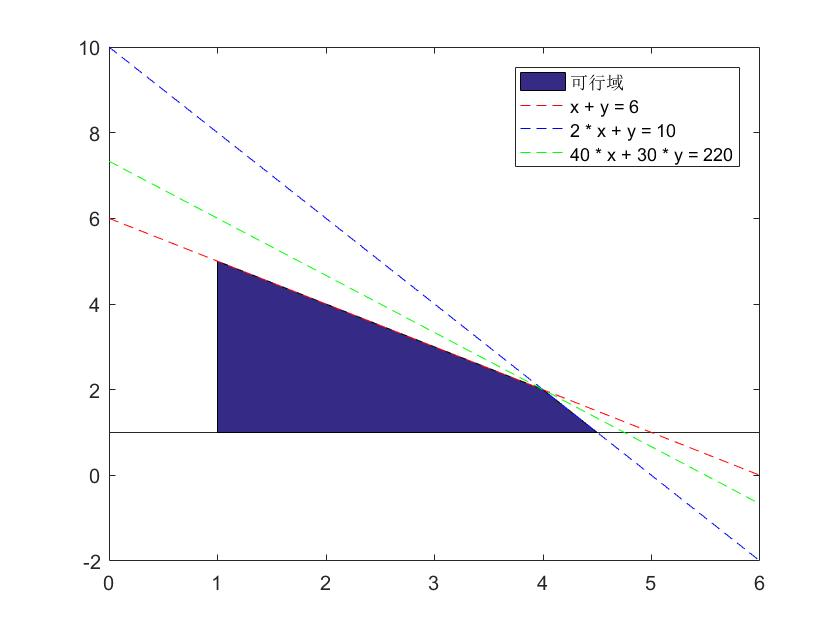
\includegraphics[width=340pt,height=270pt]{figure1.jpg}
        \caption{可行域,图解法的做法,(4,2)顶点最大}
    \end{figure}
\section{线性规划-适用题目}

\subsection{线性规划适用的赛题:} 
~题目中提到"怎样安排/分配" "尽量多/少" "最多/少" "利润最大" "最合理"等词;
\begin{itemize}
    \item[·\textcolor{blue}{生产安排}] 原材料、设备有限制、总利润最大 \par 生产两种机床,利润分别为XXX,A机器和B机器加工,两种机器工作时间...;怎样安排利润最大?(简单的线性规划,图解法即可)
    \item[·\textcolor{blue}{投资利润}] 资产配置、收益率、损失率、组合投资在、总收益最大 \par 总资金为M,共有n种资产可以配置,平均收益率...,风险损失率...,手续费...,设计组合投资方案是总收益最大,总风险最小。(多目标规划变成一个目标的线
    性规划)
    \item[·\textcolor{blue}{销售运输}] 产地、销量、销地、运费、产量、总运费最省\par 商品有m个产地和n个销售地,各产地的运费...,各销售地的需求量...,从a到b的运费...,如何使总运费最省?(0-1规划,康—希表上作业法)
    \item[·\textcolor{blue}{车辆安排}] 路线、起点终点、承载量、时间点、车次安排最合理\par 不同种类车辆有各自的承重量,工地里有多条线路,满足用工条件下,如何安排车辆使运载量最大?(整数规划,匈牙利算法)          
\end{itemize}
整数规划和0-1规划页往往默认是线性规划。
\subsection{模型变换:}
1.~规划问题为min $|x_1|+|x_2|+\cdots+|x_n|$,  s.t.$ Ax\leq b$,其中
$x={\begin{bmatrix}
    x_1&\cdots&x_n\\
\end{bmatrix}}^T$
,A,b是系数矩阵与常数向量时:
\\要把上面的问题变换成线性规划问题,只要注意到事实:对任意的 $x_i$ ,存在$
u_i , v_i > 0$满足
$$x_i=u_i-v_i,|x_i|=u_i+v_i$$
事实上,我们可以简单取出$u_i=\frac{x_i+|x_i|}{2},v_i=\frac{|x_i|-x_i}{2}$就满足上述条件,这个时候整个问题变成:
\\记$u=\begin{bmatrix}
    u_1&\cdots&u_n\\
\end{bmatrix}$,$v=\begin{bmatrix}
    v_1&\cdots&v_n\\
\end{bmatrix}$
\begin{center}
        
    目标函数\\ $\min \sum_{i=1}^{n}(u_i+v_i)$
    \\约束条件
    \\s.t.$\left\{\begin{matrix}
       A(u-v)\leq b \\
       u,v \geq 0\\
    \end{matrix}\right.$
\end{center}
    \par 2.~规划问题为$\min_{x_i}{\max_{y_i}|\varepsilon_i|}$,其中$\varepsilon_i=|x_i-y_i|$ 时:
    \\ 要把上面的问题变换成线性规划问题,只要注意到事实:当$x_0=\max_{y_i}|\varepsilon_i|$时,问题就变成了
    \begin{center}
        目标函数\\ $\min x_0$
        \\约束条件
        \\s.t.$\left\{\begin{matrix}
           x_1-y_1\leq x_0 ,&x_2-y_2\leq x_0,&\cdots ,&x_n-y_n\leq x_0\\
        \end{matrix}\right.$
    \end{center}此即我们常见的线性规划问题。
    \par 3.~规划问题为指派问题时,这个其实可以看算法大全第一章,但是那个太过抽象,我这边重新列一个好理解的:
    
    \begin{table}[h]
        \begin{center}
        \begin{tabular}[h]{|c|c|c|c|c|}
            \hline
            \diagbox{人员}{所需时间}{任务} & A &B &C &D\\
            \hline
            甲 & $a_{11}$ & $a_{12}$ & $a_{13}$ &$a_{14}$ \\
            \hline
            乙 & $a_{21}$ & $a_{22}$ & $a_{23}$ &$a_{24}$ \\
            \hline
            丙 & $a_{31}$ & $a_{32}$ & $a_{33}$ &$a_{34}$ \\
            \hline
            丁 & $a_{41}$ & $a_{42}$ & $a_{43}$ &$a_{44}$ \\
            \hline
        \end{tabular}
    \end{center}
        \end{table}
    
        一般就是这个样子,我们可以引入变量$x_{ij}$来表示是否安排第i个人完成第j项工作。
    $x_{ij}=\left\{ 
        \begin{matrix}
        1&,\mbox{安排第i人完成第j项工作}\\
        0&,\mbox{不安排第i人完成第j项工作}\\
    \end{matrix} \right.$
。随后我们就有目标函数$\min Z=a_{11}x_{11}+a_{12}x_{12}+\cdots+a_{44}x_{44}$
\\与约束条件\\(1).每个人只能做一项任务:比如甲,$x_{11}+x_{12}+x_{13}+x_{14}=1$。\\(2).每项任务只能由一个人完成:比如任务A,$x_{11}+x_{21}+x_{31}+x_{41}=1$
\\综合一下,我们有指派问题的模型:
\begin{center}
决策变量\\$x_{ij}=\left\{ 
    \begin{matrix}
    1&,\mbox{安排第i人完成第j项工作}\\
    0&,\mbox{不安排第i人完成第j项工作}\\
\end{matrix} \right.$
\\目标函数\\$\min Z=\sigma_{i}\sigma_{j}c_{ij}x_{ij}$
\\约束条件\\$\left\{ \begin{matrix}
    \sigma_{i}x_{ij}=1,j=1,2,\cdots,n\\
    \sigma_{j}x_{ij}=1,i=1,2,\cdots,n\\
    x_{ij}=1\mbox{或}0\\
\end{matrix} \right.$
\end{center}
\section{线性规划-代码实现}
    \par 贴出matlab代码求解,请结合前面整理后的式子来分别对应变量
    \begin{center}
    \begin{lstlisting}[caption={Linprog},language=Matlab]
        % Linear Programming
        f = [-40;-30];  
        A = [1,1;-1,0;0,-1;240,120];   
        b = [6;-1;-1;1200];             
        [x,fval] = linprog(f,A,b)
        fval = -fval
        \end{lstlisting}
    \end{center}
    \section{线性规划-实战演练}
    \par 国赛的难度基本上都可以说成是国家自然科学基金子课题全国征求意见稿了,你还搁这指望线性规划能解决呢。
    \\记得去看我发的算法大全第一章,这波保底进度到这,里面题我做完发出来答案(虽然不保证正确),
    这章只将线性规划,结束,收工。
\newpage
\begin{thebibliography}{99}  

    \bibitem{ref1}谢中华. MATLAB与数学建模[A].北京航空航天大学出版社[M]:科学技术协会,2021-02-14.
    \bibitem{ref2}数学建模BOOM. 线性规划(模型+适用赛题+MATLAB求解)(零基础数学建模)[M]:2021-8-30.
    \bibitem{ref3}mathworks. 非线性规划问题求解器[J]:\url{https://ww2.mathworks.cn/help/optim/ug/linprog.html#description}
    % \bibitem{ref2}陈香敏,魏伟,吴莹. “文化+人工智能”视阈下文化创意产业融合发展实践及路径研究[A]. 中共沈阳市委、沈阳市人民政府.第十七届沈阳科学学术年会论文集[C].中共沈阳市委、沈阳市人民政府:沈阳市科学技术协会,2020:4.
    % \bibitem{ref3}田晓曦,刘振鹏,彭宝权. 地方高校开展教育人工智能深度融合的路径探究[A]. 中共沈阳市委、沈阳市人民政府.第十七届沈阳科学学术年会论文集[C].中共沈阳市委、沈阳市人民政府:沈阳市科学技术协会,2020:5.
    % \bibitem{ref4}柏卓君,潘勇,李仲余.彩色多普勒超声在早期胚胎停育诊断中的应用[J].影像研究与医学应用,2020,4(18):129-131.
    % \bibitem{ref5}杨芸.我院2018年人血白蛋白临床应用调查与分析[J].上海医药,2020,41(17):34-35+74.
    
    \end{thebibliography}
\newpage
\section{数学建模算法大全第一章习题答案}
\begin{itemize}
    \item[1] 令$y=\min(\sum_{i=1}^{m}a_{i1}x_i,\sum_{i=1}^{m}a_{i2}x_i,\cdots,\sum_{i=1}^{m}a_{in}x_i)$,则问题可化为:
    \\$\max Z=y$ 
    \\s.t.$ \left\{\begin{matrix}
        \sum_{i=1}^{m}x_i=1\\
        x_i\geq 0,(i=1,2,\cdots,m)\\
        y \leq \sum_{i=1}^{m}a_{ij}x_i,(j=1,2,\cdots,n)\\
    \end{matrix}\right.$
    \item[2] 令$x_i=\frac{u_i-v_i}{2},|x_i|=\frac{u_i+v_i}{2},$则原问题可化为:
    \\$\max Z=\sum_{j=1}^{n}c_{j}(\frac{u_i+v_i}{2})$
    \\s.t.$\left\{
        \begin{matrix}
            \sum_{j=1}^{n}a_{ij}(\frac{u_i-v_i}{2})=b_i&(i=1,2,\cdots,m)\\
            u_i\geq 0\\
            v_i\geq 0\\
        \end{matrix}
    \right.$
        \item[3] 令$e_i=|y_i-(a+bx_i)|$,则原问题可化为:
        \\ $\min\sum_{i=1}^{n}e_i$,残差最小(控制代数有一个小结论,先手写一下),以下三个无约束条件下优化问题等价$$ \min\limits_{x\in\mathbb{R}^2}{\left\lVert Ax-b\right\rVert}_2^2,\min\limits_{x\in\mathbb{R}^2}{\left\lVert Ax-b\right\rVert}^2,\frac{1}{2}\min\limits_{x\in\mathbb{R}^2}{\left\lVert Ax-b\right\rVert}_2^2  $$也就是,只要有一个x满足其中一个解,那么页一定时剩下的解。
        \\那么我们的目标函数也就可以化成:
        \\$\min \mathbf{J}_1=\frac{1}{2}\sum_{i}^{n}e_i^2$
        \\s.t. 无约束条件,根据最小二乘法求出$\hat{a} ,\hat{b}$即可。
        \item[4] 简单分析:做I类产品共有:($A_1,B_1$),($A_1,B_2$),($A_1,B_3$),($A_2,B_1$),($A_2,B_2$),($A_2,B_3$)六个路径,分别设为$x_1=\sum_{i=1}^{6}x_{1i}$.
        \\同理可知,II类产品有$(A_1,B_1),(A_2,b_1)$两个路径,分别设为$x_2=\sum_{i=1}^{2}x_{2i}$
        \\则该问题可化为:
        \\$\max Z=(1.25-0.25)x_1+(2.0-0.35)x_2+(2.8-0.5)x_3-\frac{300}{6000}(5x_{11}+5x_{12}+5x_{13}+10x_{21})-\frac{321}{10000}(7x_{12}+7x_{15}+7x_{16}+9x_{22}+12x_3)-\frac{250}{4000}(6x_{11}+6x_{14}+8x_{21}+8x_{22})-\frac{783}{7000}(4x_{12}+4x_{15}+11x_3)-\frac{200}{4000}(7x_{13}+7x_{16})$
        \\s.t.$\left\{\begin{matrix}
            5x_{11}+5x_{12}+5x_{13}+10x_{21} \leq 6000\\
            7x_{14}+7x_{15}+7x_{16}+9x_{22}+12x_3\leq 10000\\
            6x_{11}+6x_4+8x_{21}+8x_{22} \leq 4000\\
            4x_{12}+4x_{25}+11x_3\leq 7000\\
            7x_{13}+7x_{23}\leq 4000\\
            x_1=x_{11}+\cdots+x_{16},x_2=x_{21}+x_{22}\\
            x_{ij}\geq 0,x_i\geq 0\\
        \end{matrix}\right.$
        可以容易求出最后的整数解:(我认为此模型解法比现在网上解法要好一点,计算值更大,契合度更高)
       $x_1=1430.00000000000
       \\x_2=500.000000000000
       \\x_3=324.000000000001
       \\x_{11}=0
       \\x_{12}=858.999999999998
       \\x_{13}=341.000000000002
       \\x_{14}=0
       \\x_{15}=0
       \\x_{16}=229.999999999999
       \\x_{17}=0
       \\x_{18}=500.000000000000$
     \item[5] 指派问题,可化为问题采用匈牙利算法:
     \\$\min Z =\Sigma_{i=1}^{4}c_{ij}x_{ij}$
     \\s.t.$\left\{ \begin{matrix}
        \Sigma_{i}x_{ij}=1,j=1,2,\cdots,n\\
        \Sigma_{j}x_{ij}=1,i=1,2,\cdots,n\\
        x_{ij}=1\mbox{或}0\\
    \end{matrix} \right.$
            \\ 可以容易求出最后的整数解(此最优解不唯一,另一解留给读者证明):
             $x_{ij}=\begin{bmatrix}
                0	&1&	0	&0\\
1	&0	&0	&0\\
0	&0	&1	&0\\
0	&0	&0	&1\\
             \end{bmatrix}
$
    \item[6]用$i=1,2$分别代表重型和轻型炸弹,$j=1,2,3,4$分别代表四个要害部位,$x_{ij}$代表投到第j要害的i种炸弹的数量,则此问题的数学模型为:\\
    
    
        $\min Z =(1-0.10)^{x_{11}}(1-0.20)^{x_{12}}(1-0.15)^{x_{13}}(1-0.25)^{x_{14}}
        (1-0.08)^{x_{21}}
        (1-0.16)^{x_{22}}(1-0.12)^{x_{23}}(1-0.20)^{x_{24}}$
        s.t.$$\left\{\begin{matrix}
            \frac{1.5 \times 450}{2}x_{11}+\frac{1.5 \ times 480}{2}x_{12}+\frac{1.5 \times 540}{2}x_{13}+\frac{1.5 \times 600}{2}x_{14}+\\\frac{1.75 \times 450}{3}x_{21}+\frac{1.75 \times 480}{3}x_{22}+\frac{2 \times 540}{3}x_{23}+\frac{2 \times 600}{3}x_{24}+\\100(x_{11}+x_{12}+x_{13}+x_{14}+x_{21}+x_{22}+x_{23}+x_{24})\leq 48000\\
            x_{11}+x_{12}+x_{13}+x_{14} \leq 32\\
            x_{21}+x_{22}+x_{23}+x_{24} \leq 48\\
            x_{ij}\geq 0 \qquad i=1,2;j=1,\cdots,4\\
        \end{matrix}\right.$$
虽然目标函数非线性,但是$\min Z$可用$\max \lg{\frac{1}{Z}}$,因此目标函数变成
\\$\max Z =0.0457x_{11}+0.0969x_{12}+0.0704x_{13}+0.1248x_{14}+0.0362x_{21}+\\0.0656x_{22}+0.0554x_{23}+0.0969x_{24}$
\item[7]直接给解:$x_1 =
4.0000
,x_2=1.0000
,x_3=9.0000
\\Z=2.0000$
\item[8]直接给解:$u_1=
0.5000,
v_1=0.0000,
u_2=0.0000,
v_2=0.0000,
u_3=0.0000,
v_3=0.0000,
u_4=0.0000,
v_4=0.5000,$
\\也就是$
x_1=0.25,x_2=0,x_3=0,x_4=-0.25;
Z =1.2500$

\item[9]分别给出决策变量:用$i=1,2,3,4$分别表示货物1,货物2,货物3和货物4;$j=1,2,3$分别表示前舱,中舱和后舱。设$x_{ij}(i=1,2,3,4;j=1,2,3)$表示第i种货物装载第j个货舱内的重量,$w_j,v_j(j=1,2,3)$分别表示第j个舱的重量限制和体积限制,$a_i,b_i,c_i(i=1,2,3,4)$分别表示可以运输的第i种货物的重量,单位重量所占的空间和单位货物的利润,则
\par (1).目标函数为\par $\max Z=c_1\sum\limits_{j=1}^3x_{1j}+c_2\sum\limits_{j=1}^3x_{2j}+c_3\sum\limits_{j=1}^3x_{3j}+c_4\sum\limits_{j=1}^3x_{4j}\\=\sum\limits_{i=1}^4\sum\limits_{j=1}^3c_ix_{ij}$
\par (2).约束条件为\par s.t.$\left\{\begin{matrix}
    \sum\limits_{j=1}^3x_{ij}\leq a_i,i=1,2,3,4\\
    \sum\limits_{i=1}^4x_{ij}\leq w_j,j=1,2,3\\
    \sum\limits_{i=1}^4b_ix_{ij}\leq v_i,j=1,2,3\\
    \frac{\sum\limits_{i=1}^4x_i1}{10}=\frac{\sum\limits_{i=1}^4x_i2}{16}=\frac{\sum\limits_{i=1}^4x_i3}{8}\\
\end{matrix}\right.$
\\最终有解:$x =
4.48353476103949e-13      \qquad    14.9999999999999      \qquad    15.9473684210523      \\ \qquad   3.05263157894734
\\y =121515.789473684$

\end{itemize}
\end{document}